\section{Standard di qualità}

\subsection{ISO/IEC 15504}
ISO/IEC 15504, conosciuto anche come SPICE (\textit{Software Process Improvement and Capability Determination}), è lo standard internazionale usato per valutare la qualità dei processi software e perseguirne il miglioramento continuo. La qualità di ogni processo viene valutata oggettivamente mediante la misurazione della capacità dello stesso tramite specifici attributi. \\
Lo standard ISO/IEC 15504 definisce un modello di riferimento che si suddivide in:
\begin{itemize}
	\item{dimensione del processo;}
	\item{dimensione della capacità.}
\end{itemize}

\subsubsection{Dimensione del processo}
La \textit{process dimension} divide i processi in cinque categorie:
	\begin{itemize}
		\item{Customer/Supplier;}
		\item{Engineering;}
		\item{Supporting;}
		\item{Management;}
		\item{Organization.}
	\end{itemize}

\subsubsection{Dimensione della capacità}
Per ogni processo, ISO/IEC 15504 definisce un livello di maturità basato sulla scala rappresentata di seguito:

	\rowcolors{2}{lightRowColor}{darkRowColor}
	\begin{longtable}{ 
		>{\centering}p{0.4\textwidth} 
		>{\centering\arraybackslash}p{0.5\textwidth}}
		\caption {Scala di maturità dello standard ISO/IEC 15504}		\\
		\coloredTableHead
		\textbf{\color{white}Livello} &
		\textbf{\color{white}Nome}
		\tabularnewline  
		\endhead
		% Contenuto della tabella
		5 & Optimizing process \\
		4 & Predictable process \\
		3 & Established process \\
		2 & Managed process \\
		1 & Performed process \\
		0 & Incomplete process
	\end{longtable}	
	
La capacità (o maturità) di ciascun processo viene misurata tramite gli attributi descritti di seguito:
	
	\rowcolors{2}{lightRowColor}{darkRowColor}
	\begin{longtable}{ 
		>{\centering}p{0.4\textwidth} 
		>{\centering\arraybackslash}p{0.5\textwidth}}
		\caption {Attributi per la misurazione della capacità dello standard ISO/IEC 15504}		\\
		\coloredTableHead
		\textbf{\color{white}Appartenenza al livello ed identificativo} &
		\textbf{\color{white}Nome}
		\tabularnewline  
		\endhead
		% Contenuto della tabella
		1.1 & Process Performance \\
		2.1 & Performance Management \\
		2.2 & Work Product Management \\
		3.1 & Process Definition \\
		3.2 & Process Deployment \\
		4.1 & Process Measurement \\
		4.2 & Process Control \\
		5.1 & Process Innovation \\
		5.2 & Process Optimization 
	\end{longtable}	
	
Ciascun attributo consiste di una o più pratiche generiche che aiutano nella fase di valutazione. Inoltre, ciascun attributo è valutato secondo una scala a quattro valori (N-P-L-F):

	\rowcolors{2}{lightRowColor}{darkRowColor}
	\begin{longtable}{ 
		>{\centering}p{0.4\textwidth} 
		>{\centering\arraybackslash}p{0.5\textwidth}}
		\caption {Scala di valutazione degli attributi dello standard ISO/IEC 15504}		\\
		\coloredTableHead
		\textbf{\color{white}Stato} &
		\textbf{\color{white}Range di valori corrispondenti}
		\tabularnewline  
		\endhead
		% Contenuto della tabella
		Not achieved & 0 - 15\% \\
		Partially achieved & >15 - 50\%  \\
		Largely achieved & >50 - 85\% \\
		Fully achieved & >85 - 100\% \\
	\end{longtable}	

La valutazione viene fatta sulla base di evidenze oggettive acquisite durante la fase di assessment. La figura di seguito mostra la relazione tra livello di maturità, attributi di misurazione e relativa scala di valutazione nell'attività di valutazione della qualità di processo.

\begin{figure}[H]
		\centering
		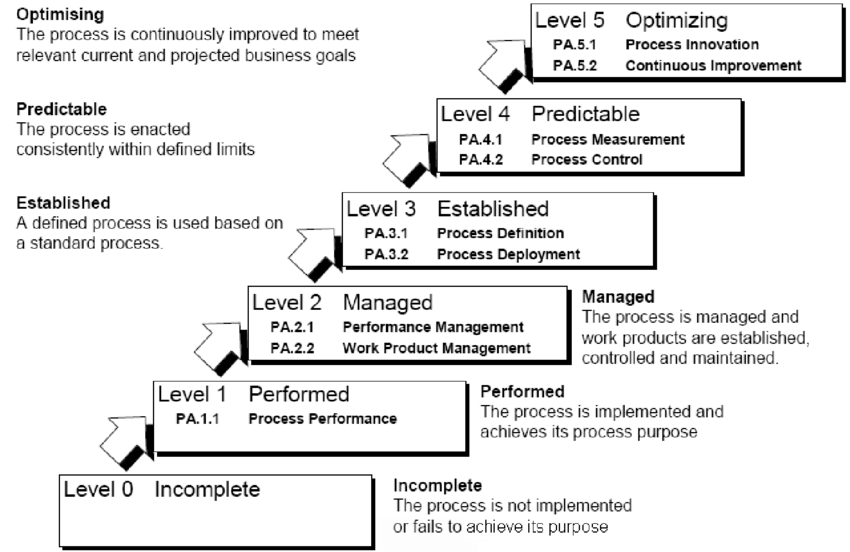
\includegraphics[scale=0.5]{./res/img/ISO_IEC_15504.png}
		\caption[Modello ISO/IEC 15504]{SPICE Capability (fonte: Janos Ivanyos, \texttt{researchgate.net})}
\end{figure}
\pagebreak

\subsection{Ciclo di Deming}
Il ciclo di Deming (o ciclo di PDCA, acronimo dall'inglese di \textit{Plan-Do-Check-Act}) è un metodo di gestione iterativo utilizzato per il controllo ed il miglioramento continuo dei processi e, di riflesso, anche dei prodotti da questi risultanti. 
Il ciclo di Deming è strutturato in quattro fasi, come illustrate di seguito:
	\begin{figure}[H]
		\centering
		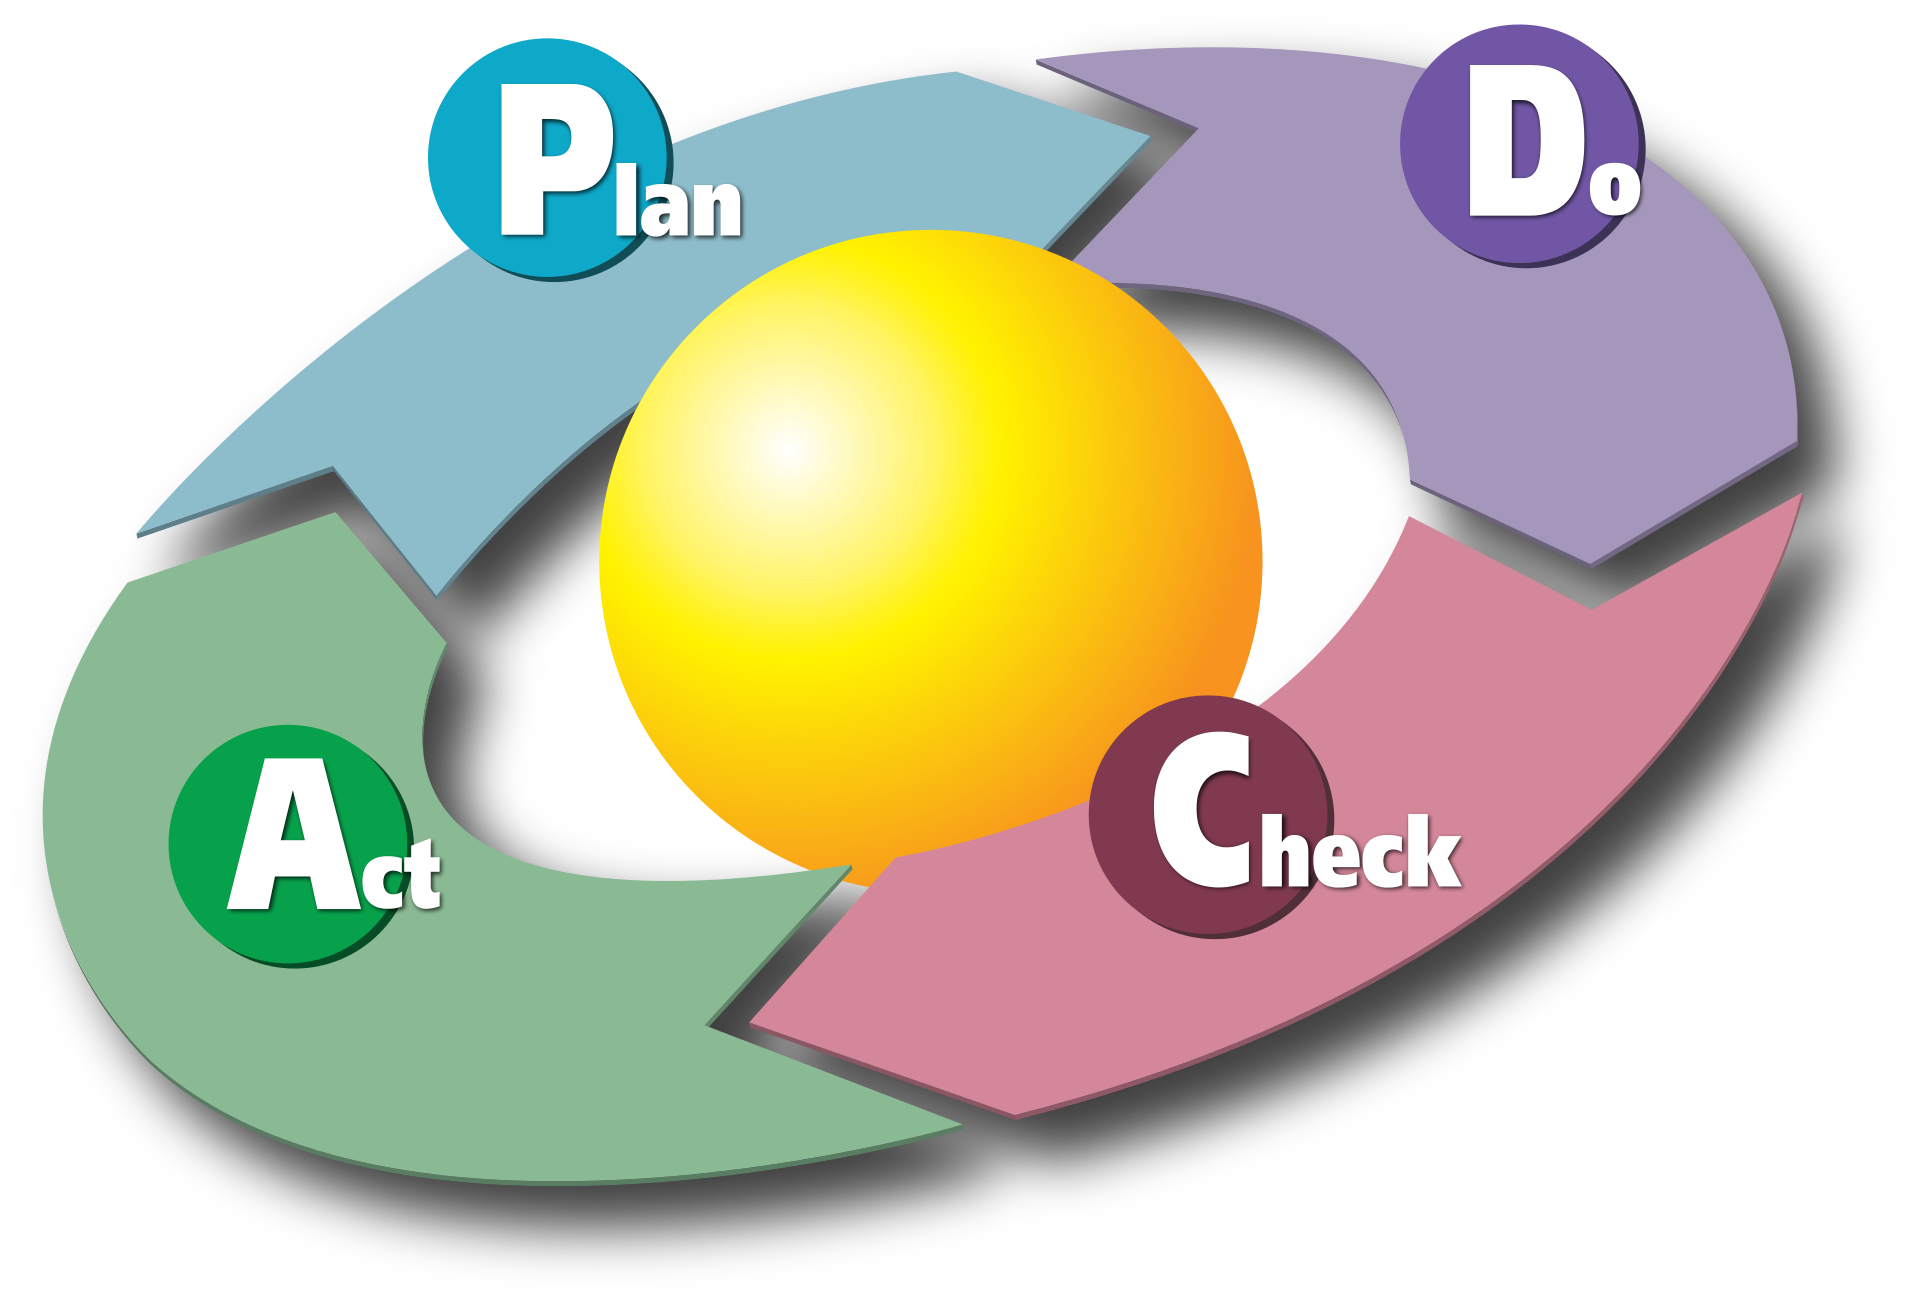
\includegraphics[scale=0.1]{./res/img/PDCA.png}
		\caption[Ciclo PDCA]{Ciclo PDCA per il miglioramento continuo (fonte: Wikipedia)}
	\end{figure}

\begin{enumerate}
	\item{\textbf{Plan}: è la fase di pianificazione in cui vengono stabiliti gli obiettivi ed i processi necessari a raggiungerli. In questa fase vengono definite tutte le attività da svolgere, le risorse da assegnarvi e le scadenze da rispettare;}
	\item{\textbf{Do}: è la fase di esecuzione del programma precedentemente stilato, dapprima -se possibile- in contesti circoscritti. E' possibile ed auspicabile in questa fase raccogliere dati utili alle fasi di \textit{Check} e \textit{Act};}
	\item{\textbf{Check}: è la fase di controllo per accertarsi che la fase \textit{Do} sia stata eseguita in accordo con ciò che era stato deciso nella fase \textit{Plan}. In questa fase vengono anche studiati i risultati confrontandoli con quelli attesi;}
	\item{\textbf{Act}: è la fase di attuazione, che permette di rendere definitivi i processi i cui esiti sono stati positivi o apportare modifiche migliorative in caso contrario.}
\end{enumerate}
I quattro punti sopra indicati costituiscono una sequenza logica che viene ripetuta finché l'obiettivo finale non è raggiunto.
\pagebreak

\subsection{ISO/IEC 9126}
ISO/IEC 9126 è lo standard internazionale usato per valutare la qualità del software. Esso è articolato in quattro parti:
\begin{enumerate}
	\item{modello per la qualità del software, che a sua volta è suddiviso in:}
	\begin{itemize}
		\item{modello per la qualità esterna ed interna;}
		\item{modello per la qualità in uso;}
	\end{itemize}
	\item{metriche per la qualità interna;}
	\item{metriche per la qualità esterna;}
	\item{metriche per la qualità in uso.}
\end{enumerate}

	\subsubsection{Modello per la qualità del software}
	\begin{figure}[H]
		\centering
		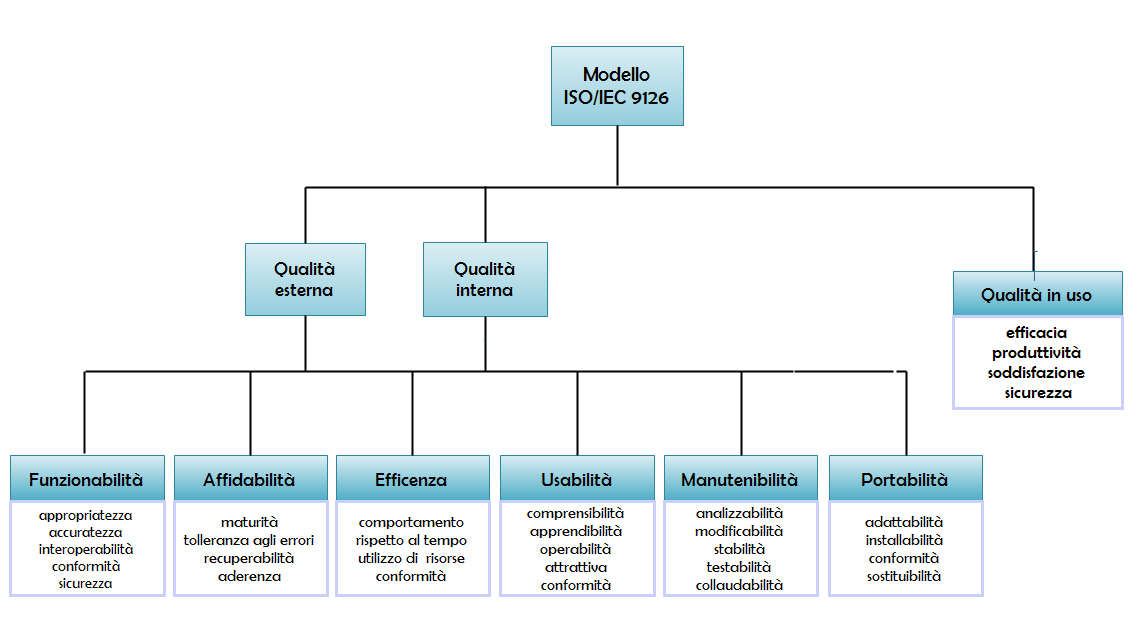
\includegraphics[scale=0.5]{./res/img/ISO_IEC_9126.png}
		\caption[Modello ISO/IEC 9126]{Modello ISO/IEC 9126 (fonte: Wikipedia)}
	\end{figure}
	
	\subsubsubsection{Modello per la qualità esterna ed interna}
	Il modello per la definizione della qualità interna ed esterna è composto da sei caratteristiche generali e varie sotto caratteristiche misurabili attraverso delle metriche. Tali caratteristiche sono:
	
	\subsubsubsection*{Funzionalità}
	E' la capacità del software di fornire funzioni che soddisfano esigenze stabilite nell'\textit{\AdR{}} e che permettono di operare in condizioni specifiche. Questa capacità si traduce nelle seguenti sotto caratteristiche:
	\begin{itemize}
		\item{\textbf{appropriatezza}: capacità di fornire funzioni appropriate per attività specifiche che permettano di raggiungere gli obiettivi prefissati;}
		\item{\textbf{accuratezza}: capacità di fornire risultati corretti e con la precisione richiesta;}
		\item{\textbf{interoperabilità}: capacità di interagire con uno o più sistemi specificati;}
		\item{\textbf{conformità}: capacità di aderire a standard rilevanti al settore in esame;}
		\item{\textbf{sicurezza}: capacità di proteggere informazioni e dati.}
	\end{itemize}
	
	\subsubsubsection*{Affidabilità}
	E' la capacità del software di mantenere uno dato livello di prestazioni quando usato in specifiche condizioni. Questa capacità si traduce nelle seguenti sotto caratteristiche:
	\begin{itemize}
		\item{\textbf{maturità}: capacità di evitare il verificarsi di errori o malfunzionamenti in fase di esecuzione;}
		\item{\textbf{tolleranza agli errori}: capacità di mantenere livelli predeterminati di prestazioni anche in presenza di malfunzionamenti o errori;}
		\item{\textbf{recuperabilità}: capacità di ripristinare il livello di prestazioni e di recupero delle informazioni rilevanti in seguito ad un malfunzionamento;}
		\item{\textbf{aderenza}: capacità di aderire a standard e regole inerenti all'affidabilità.}
	\end{itemize}
	
	\subsubsubsection*{Efficenza}
	E' la capacità del software di eseguire le funzioni prefissate minimizzando il tempo necessario e sfruttando al meglio le risorse disponibili. Questa capacità si traduce nelle seguenti sotto caratteristiche:
	\begin{itemize}
		\item{\textbf{nel tempo}: capacità di fornire appropriati tempi di risposta;}
		\item{\textbf{nello spazio}: capacità di utilizzare un appropriato numero di risorse.}
	\end{itemize}
	
	\subsubsubsection*{Usabilità}
	E' la capacità del software di essere capito, appreso, usato ed accettato positivamente dall'utente. Questa capacità si traduce nelle seguenti sotto caratteristiche:
	\begin{itemize}
		\item{\textbf{comprensibilità}: capacità di essere chiaro riguardo le proprie funzionalità ed il proprio utilizzo;}
		\item{\textbf{apprendibilità}: capacità di essere facilmente apprendibile;}
		\item{\textbf{operabilità}: capacità di permettere all'utente di raggiungere i suoi scopi e controllarne l'uso;}
		\item{\textbf{attrattività}: capacità di essere piacevole per l'utente che ne fa uso;}
		\item{\textbf{conformità}: capacità di aderire a standard o convenzioni relativi all'usabilità.}
	\end{itemize}

	\subsubsubsection*{Manutenibilità}
	E' la capacità del software di essere modificato includendo correzioni, miglioramenti od adattamenti. Questa capacità si traduce nelle seguenti sotto caratteristiche:
	\begin{itemize}
		\item{\textbf{analizzabilità}: capacità di essere facilmente analizzato al fine di individuare un errore;}
		\item{\textbf{modificabilità}: capacità di essere agevolmente modificato nel codice, nella progettazione o nella documentazione;}
		\item{\textbf{stabilità}: capacità di evitare effetti indesiderati a seguito di una modifica;}
		\item{\textbf{testabilità}: capacità di essere facilmente testato al fine di validare le modifiche apportate.}
	\end{itemize}

	\subsubsubsection*{Portabilità}
	E' la capacità del software di essere trasportato da un ambiente hardware/software ad un altro seguendo le evoluzioni tecnologiche. Questa capacità si traduce nelle seguenti sotto caratteristiche:
	\begin{itemize}
		\item{\textbf{adattabilità}: capacità di essere facilmente adattato a differenti ambienti operativi senza applicare modifiche;}
		\item{\textbf{installabilità}: capacità di essere installato in uno specifico ambiente;}
		\item{\textbf{conformità}: capacità di aderire a standard e convenzioni relative alla portabilità;}
		\item{\textbf{sostituibilità}: capacità di essere utilizzato al posto di un altro software per svolgere gli stessi compiti nello stesso ambiente.}
	\end{itemize}
	
	\subsubsubsection{Modello per la qualità in uso}
	Il modello per la definizione della qualità in uso elenca quattro caratteristiche generali che permettono agli utenti di ottenere specifici obiettivi. Tali caratteristiche sono:
	\begin{itemize}
		\item{\textbf{efficacia}: capacità del software di permettere agli utenti di raggiungere gli obiettivi specificati con accuratezza e completezza;}
		\item{\textbf{produttività}: capacità del software di essere efficiente rispetto alle risorse necessarie;}
		\item{\textbf{soddisfazione}: capacità del software di soddisfare gli utenti;}
		\item{\textbf{sicurezza}: capacità del software di avere dei livelli di rischio accettabili rispetto a danni nei confronti di persone, apparecchiature e ambiente operativo.}
	\end{itemize}
	
	\subsubsection{Metriche per la qualità interna}
	La qualità interna viene rilevata tramite analisi statica, ovvero le metriche scelte vengono applicate a software non eseguibile e permettono di individuare eventuali problemi che potrebbero influire sulla qualità finale del prodotto. Le misure effettuate permettono di prevedere il livello di qualità esterna ed in uso del prodotto finale.
	
	\subsubsection{Metriche per la qualità esterna}
	La qualità esterna viene rilevata tramite analisi dinamica. Le metriche sono applicate al software in esecuzione e ne misurano il comportamento attraverso attività di test in funzione degli obbiettivi prefissati.
	Idealmente la qualità esterna determina la qualità in uso.
	
	\subsubsection{Metrica per la qualità in uso}
	Si tratta di metriche applicabili solo al prodotto finito ed in uso in condizioni reali. La qualità in uso viene raggiunta solo se è stato raggiunto sia il livello di qualità interna che di qualità esterna.